\vspace{-0.5cm}
\section{Dreiphasenwechselstrom und Drehfelderzeugung} \label{SternDreieck}
\vspace{-0.25cm}
    \renewcommand{\arraystretch}{1}
    \begin{tabular}[b]{| C{4cm} | P{9cm} | P{5cm} |}
    	\hline
        \textbf{Sternspannungen} &
        $U_U(t) = U_m\cdot\sin\left(\omega t\right)$ \newline \newline
        $U_V(t) = U_m\cdot\sin\left(\omega t - \dfrac{2\pi}{3}\right)$ \newline \newline
        $U_W(t) = U_m\cdot\sin\left(\omega t - \dfrac{4\pi}{3}\right)$ &
        $U_U, U_V, U_W \,\widehat{=}$ den Spannungen zwischen dem Neutralleiter und dem Aussenleiter\newline
        oft 230V
        \\ \hline
         
        \textbf{Stern-Dreieck Umwandlung}&
        \vspace{0.025cm}$ U_Y= \dfrac{U_\Delta}{\sqrt{3}} $\qquad
        $ I_Y= \dfrac{I_\Delta}{\sqrt{3}} $ \qquad
        $ I_Y = I_{12} $\newline
        \vspace{0.025cm}$ M_Y= \dfrac{M_\Delta}{3} $ \qquad
        $ P_Y = \dfrac{P_\Delta}{3}$ \qquad
        $ U_\Delta = U_{12} $&
        $U = Strangspannung [V] $\newline
        $I = Strangstrom [A] $\newline
        $M = Motormoment [Nm]$ \newline 
        $P = Leistung$
        \\ \hline                
        \textbf{Verkettete Spannung} & 
        $U_{UV}(U_{12}), U_{VW}(U_{23}), U_{WU}(U_{31})$&
        oft 400V
        \\ \hline
    \end{tabular}
    \begin{center}
        \vspace{-0.4cm}
    \begin{minipage}{0.8\linewidth}
    	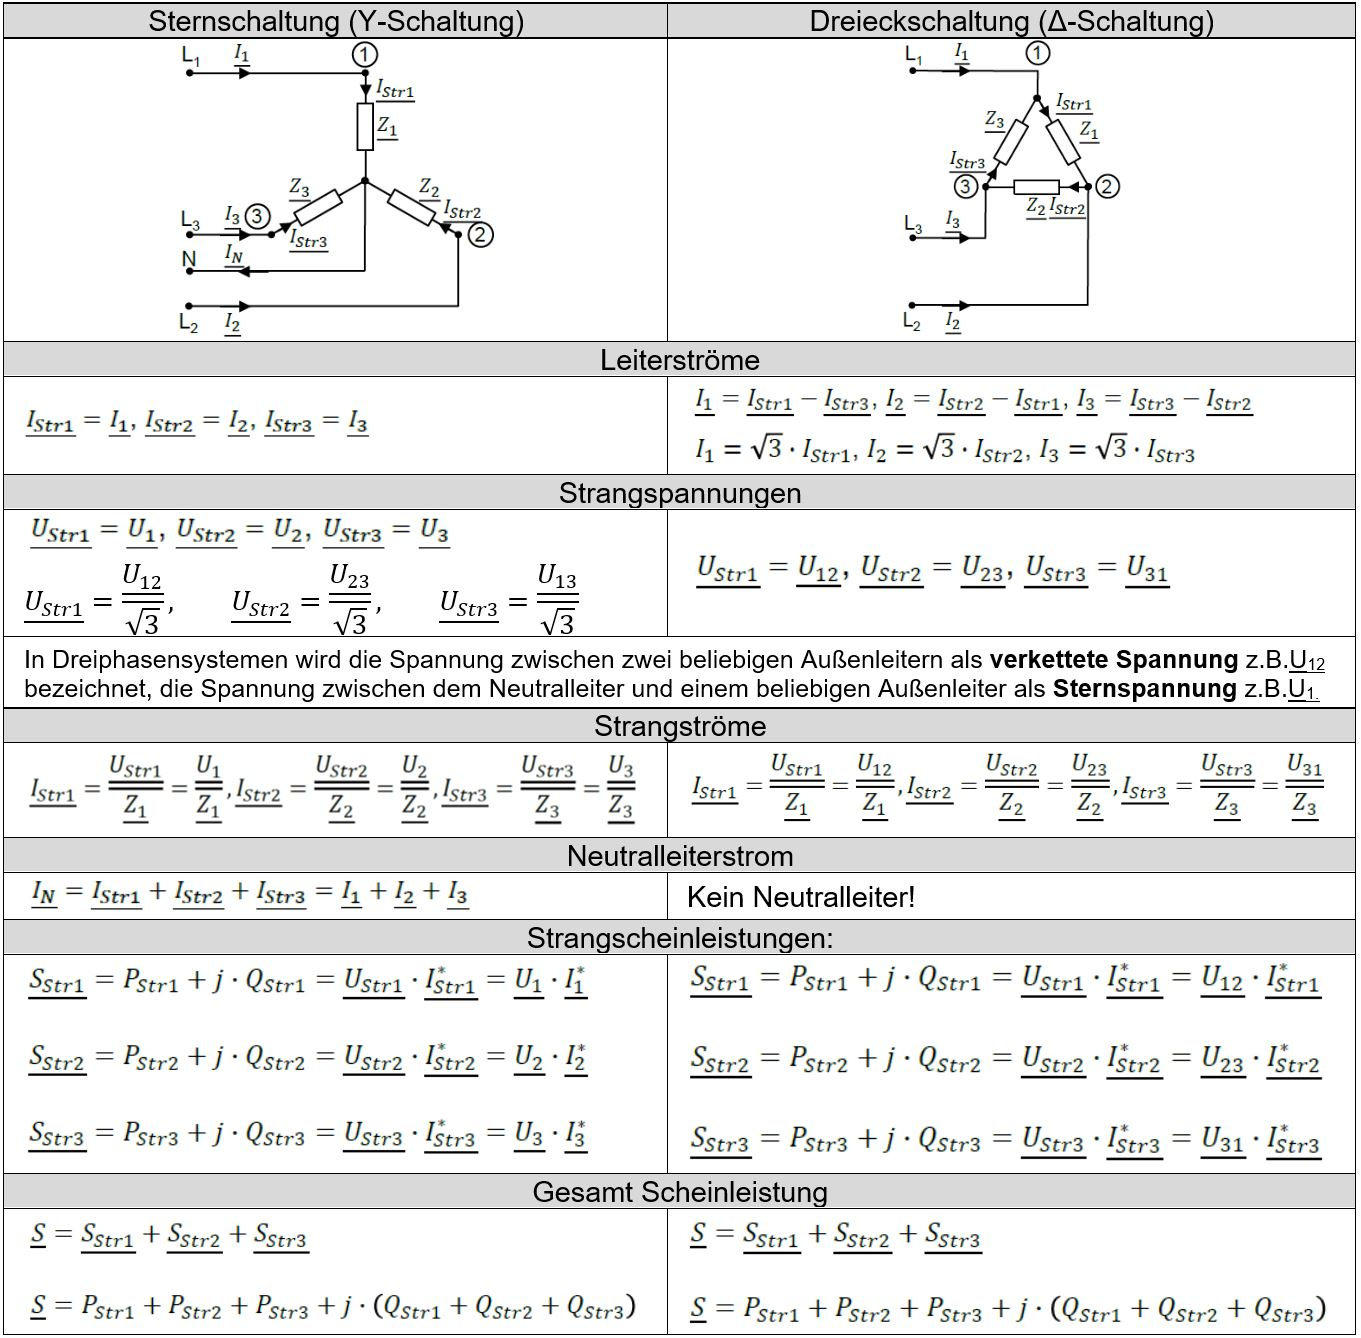
\includegraphics[width=\linewidth]{images/SternDreieck}
        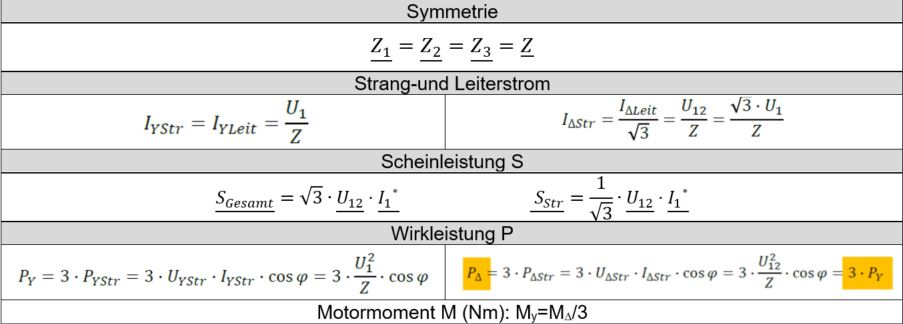
\includegraphics[width=\linewidth]{images/SternDreieckSym}
    \end{minipage}
\end{center}
%    \begin{minipage}[b]{0.4\linewidth}
%    	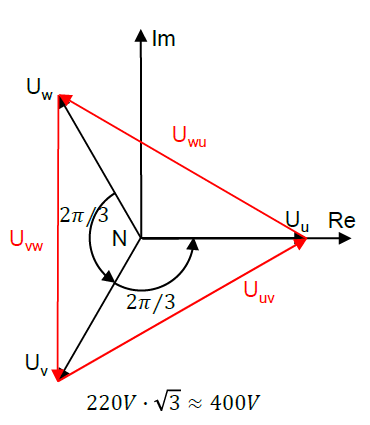
\includegraphics[width = 3.5cm]{images/Spg}
%    \end{minipage}
%    \begin{minipage}[b]{0.6\linewidth}
%    	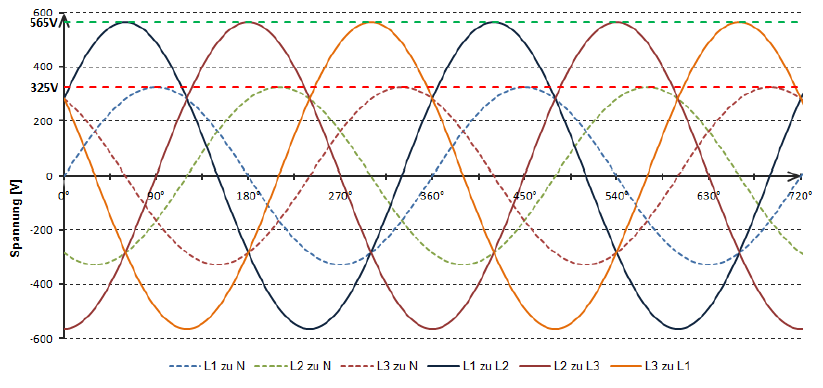
\includegraphics[width = 9cm]{images/Spg1}
%    \end{minipage}
    \clearpage
    \pagebreak
